\section{依赖与系统状态} \label{Sec.status}

系统状态与资源等涉及副作用的方面,$\amlh$ 有两种方法解决。
%
%至今的论述一直未曾讨论系统状态的处理。纯粹的λ演算固然美好,但并不适于处理系统状态与副作用
%(side affect),这也是为何目前学界普遍使用状态机以有效地处理指针、文件资源等系统状态。
%
%对此 $\amlh$ 有两种方法解决。

\subsection{状态与计算分离}

第一种方案是状态与计算分离的模型,是使用请求-响应模型(request-response),
将程序分割成下层平台与上层计算过程两个部分,令生存期管理(life time manage)、
数据持久化(data persistence)由下层的平台管理,
而计算过程只负责计算响应与对状态的修改指令,在计算中无法修改系统状态,
仅是将状态修改指令输出,而后由下层平台执行再发生实际的状态改变,
于是整个程序退化为纯粹的数值计算。

\begin{figure}[!h]
\centering
\begin{tikzpicture}
    \draw [ultra thick] (1,1) rectangle (3,2);
    \draw [->, thick] (0,3) -- (1.8,2.2);
    \draw [->, thick] (1.8,0.8) -- (0,0);
    \node at (2,1.5) {平台}; \node at (1.4,3) {请求};
    \node at (1.4,0.2) {响应};
    \draw [ultra thick] (5,1.5) ellipse (1 and 0.5);
    \node at (5,1.5) {计算过程};
    \draw [->, thick] (2,2.2) to [out=45,in=125] (5,2.1);
    \draw [<-, thick] (2,0.8) to [out=-45,in=-125] (5,0.9);
    \node [right] at (5.5, 2.5) {请求与当前状态};
    \node [right] at (5.5, 0.5) {响应与状态转移指令};
    \node at (-0.5, 1.5) {执行状态转移};
    \node at (9, 1.5) {仅计算响应与状态转移指令};
\end{tikzpicture}
\caption{状态与计算分离}
\end{figure}

这其实是构建了状态机,但将状态机中不涉及实际的状态转移的仅是对状态如何转移的计算,
分离出来。这种方法将状态转移抽象成一种指令,而计算部分是纯粹地对这些指令计算,计算出
根据用户逻辑当下该进行如何的状态转移并将这些转移以指令的方式输出,交给下层的平台,
再由平台实际地执行状态转移。于是对于计算过程,状态转移就退化成彻底的数值计算。

具体来说,即计算过程的输入中增加一个表示状态的只读参数,输出中增加一个状态修改指令的列表。
现在我们形式地描述这一机制。

\begin{defin}[系统状态] 逻辑类型 status 表示所有的系统状态,由具体实现具体定义。
\end{defin}

同样本节描述的{\it 状态与计算分离}也是一种框架,
根据具体应用场景可以给出不同的 status 类型的具体定义。
不同的 status 定义不影响状态与计算分离理论。

\begin{defin}[状态转移] HOL 逻辑上的类型 transition\_operation 表示所有系统状态转移指令,
即是各种对系统状态的修改指令。同样也是可以定制的,而后具体实现时再给出的。
唯一的要求是
\[ \abs{\mathrm{transition\_operation}} \leq \abs{\mathrm{phenomenon}} \]
这是为了之后虚构 transition\_operation 的理解。
\end{defin}

\begin{defin}[状态的理解] 
\[ (\mathbf{SI} : \mathrm{status} \rightarrow \itp{\mathrm{status}}) \coloneqq
    \mathbf{I1} \]

其中 $\mathbf{I1}$ 是样例\ref{exam.I1}中描述的单元素理解。在样例\ref{exam.I1}中
论述了,$\mathbf{I1}$ 只有一个本质元素而不会在编译结果中实质地出现。
这样以 $\mathbf{SI}$ 为理解的状态参数实质是一种伪参数,并不会在编译结果中实质地出现。

同样有如下简写记号
    \[ \mathbf{SI}\ s \coloneqq \mathbf{SI}_s \]
\end{defin}

状态的相关读取操作可以按如下框架引入。

假设 $f : \mathrm{status} \rightarrow \mathrm{some\_resource}$ 表示所期望构建的
某个状态读取操作的本质对应,亦即$f$是一个逻辑函数,将逻辑表示的状态即$status$类型表示的
逻辑结构映射到逻辑表示的某种资源,且$R$是预先构建的此资源类型的理解,
$cond : \mathrm{status} \rightarrow \mathrm{bool}$ 是某种条件且满足
    \[ \forall s.\ cond\ s \Rightarrow f\ s \in \mathbf{Se}_R \]
那么可以由虚构基元律引入满足如下性质的基元操作 $op$ 
    \[ \forall s.\ op \proctr{\mathbf{SI}_s|R}{cond} f\]

\begin{defin}[状态转移的理解] 由虚构引入 transition\_operation 的理解 $\mathbf{TI}$,
    并虚构地引入相应的构造函数。
    \[ \mathbf{V}_\mathbf{TI} \]
并利用样例\ref{exam.LI}中定义的列表理解$\mathbf{LI}$,状态转移列表的理解即是
$\mathbf{LI}\ \mathbf{TI}$,由公式 \ref{V.LI} 得到 $\mathbf{V}_\mathbf{LI\ TI}$
\end{defin}

\begin{example}[区块链环境下的示例] 假设 transition\_operation1 被如下定义。
\[ \mathrm{transition\_operation1} \Coloneqq \mathbf{WriteChain}\ \mathrm{number}\ 
    \mathrm{number}\]
且同样地假设 $\abs{\mathrm{phenomenon}} = \aleph_1$,
显然亦有 $\abs{\mathrm{transition\_operation1}} = \aleph_1$
    \[ \abs{\mathrm{transition\_operation1}} \leq \abs{\mathrm{phenomenon}} \] 
于是可以虚构定义 transition\_operation1 的理解,记为 $\mathbf{TI1}$
    \[ \mathbf{V}_\mathbf{TI1}\ \land\ (\mathbf{Se}_\mathbf{TI1} = 
    \mathrm{transition\_operation1}) \]
且虚构定义基元操作 $\mathbf{OpWriteChain}$
    \[ \mathbf{OpWriteChain} \proctr{\mathcal{N}|\mathcal{N}|\mathbf{TI1}}{\K (\K \T)}
    \mathbf{WriteChain} \]
\end{example}

\begin{defin}[响应] $\amlh$ 中的过程可以接受多个参数却只能返回一个结果,故而引入响应理解
$\mathbf{Rsp} : \itp{\alpha} \rightarrow \itp{(\alpha,\ \mathrm{transition\_operation\ list})}$
将数值结果与状态转移指令联合起来。
    \[ \mathbf{Rsp}\ i \coloneqq i \cdot (\mathbf{LI\ TI})\]
$\mathbf{Rsp}$ 并不是什么新鲜事物,仅仅是将定义\ref{Def.I*}中的理解合并包装了起来。
\end{defin}

\begin{defin}[满足状态与计算分离模型的过程] 一个过程$f_p$ 满足计算与状态分离模型当且仅当
    其具有如下形式的超越对应关系。
    \[ f_p \proctr{\cdots|\mathbf{SI}|\mathbf{Rsp}_l}{cond} f_e \]
其中 $f_e$ 的类型具有形式 $\cdots \rightarrow \mathrm{status} \rightarrow 
    (\alpha,\ \mathrm{transition\_operation\ list})$,
于是 $f_e$ 清晰地揭示出过程$f_p$ 如何对系统状态造成改变以及系统状态转移的抽象意义。
更进一步,$f_e$ 可被用于任意地对$f_p$的系统状态转移的分析与研究,
且这种分析并不困难,因为 $f_e$ 是抽象且易于分析的。
\end{defin}

\subsection{状态纳入{\phew}}

也可以不将计算与状态转移分离,而是用一种基于单源单汇有向无环网络流的
结构将状态数值化而纳入{\phew}中,即令{\phew}包含状态,那么{\phew}上的函数或者说
$\amlh$ 上的过程就可以进行状态转移的计算。

这一模型中状态被抽象为各个分立无关的资源,状态是各资源到其当前状态的映射。

\begin{equation} \label{Def.Stat}
\begin{split} 
& \textnormal{status} \Coloneqq \textnormal{ResKey} \mapsto \textnormal{ResStatus} 
 \\
& \textnormal{ResKey} \Coloneqq \textnormal{history} \quad\quad \textnormal{ResStatus} \Coloneqq \textnormal{number} 
\end{split}
\end{equation}

其中 $\textnormal{ResKey}$ 用于标识系统资源,类型 history 将在下文详细论述;$\textnormal{ResStatus}$ 
表示资源的状态,用自然数表示。一切资源的状态都是可以用一个自然数表示的,
尽管这个自然数可能非常大。事实上整个计算机的内存状态都可以用一个巨大的自然数表示。
这自然数有多大并不重要,因为形式上的符号分析实际不需要将其具体数值计算出来。
而实际地形式分析中也不需要直接面对自然数,对不同种类的资源可以定义专用的
逻辑类型以形式分析,而只需要增加一个到自然数的单射函数即可转换到自然数。
自然数表示资源状态的唯一限制是资源状态集的势不得超过$\aleph_1$,
本文认为这问题不大,大多数状态都是有限的或同构于自然数集。

引入这点后可以开始正式地论述,以过往每一次对系统资源的读取与修改
等各种历史操作为节点,以偏序的依赖关系为边,
并设立一个无意义的节点$\mathbf{HGenerator}$为源点,
以给定的节点为汇点,构成一张有向无环单源单汇网络流,称作历史流。

每一个节点都是一个计算,
$\amlh$不显式地区分线程,而是基于依赖关系,依赖关系的存否
首先决定并行还是串行,偏序方向进而决定串行的执行次序。

系统资源的访问直接构成状态依赖,故而依赖关系
为边构成的图是很清晰恰当的,图中的每一条链就是
一条串行的执行次序(见图\ref{fig:His1})。
而每一张图都记录了汇点之前所有操作的历史与依赖关系,
可以追溯这些历史轻松还原出
汇点上的系统状态。即经历了汇点之前所有点的操作,
并按由边记录的依赖顺序执行后的系统状态。
而这一结构实际上将汇点时的系统状态数值化,
以单源单汇网络流为数据结构的值。

\begin{align} 
\textnormal{fee} \Coloneqq \quad & \textnormal{number} \tag{Def.fee} \label{Def.fee} \\
\textnormal{label} \Coloneqq \quad & \mathbf{Label}\ \textnormal{string}\ \textnormal{fee} 
\tag{Def.label} \label{Def.label} \\
\begin{split} \label{Def.history}
\textnormal{history} \Coloneqq \quad & \mathbf{HGenerator} \quad | 
\quad \mathbf{HSpend} \ \textnormal{label} \ \textnormal{history} \\
& | \quad \mathbf{HWrite}\ \textnormal{history}\ \textnormal{number}\ \textnormal{history}
\\ & | \quad \mathbf{HRead}\ \textnormal{history}\ \textnormal{history}
\\ & | \quad \mathbf{HMerge}\ \textnormal{history}\ \textnormal{history}
\end{split} \tag{Def.history} \\
\mathbf{Label}\ name\ cost \quad & \colon \quad \text{名为$name$ 消耗 $cost$ 费用的标号
} \notag \\
\textnormal{history} \quad & \colon \quad \text{历史流上的节点} \notag \\
\mathbf{HGenerator} \quad & \colon \quad \text{历史流的源点} \notag \\
\mathbf{HSpend}\ l\ h \quad & \colon \quad \text{在$h$后接上标号$l$} \notag \\
\mathbf{HWrite}\ \rho\ x\ h \quad & \colon \quad \text{在$h$后接上对资源$\rho$写入$x$} \notag \\
\mathbf{HRead}\ \rho\ h \quad & \colon \quad \text{在$h$后接上对资源$\rho$读取} \notag \\
\mathbf{HMerge}\ h_1\ h_2 \quad & \colon \quad \text{同时连接自$h_1$与$h_2$的节点,表示
线程的合并} \notag
\end{align}

其中$\mathbf{HSpend}$ 与 $\mathbf{HMerge}$ 是两种技术性节点。
$\mathbf{HWrite}$, $\mathbf{HRead}$, $\mathbf{HSpend}$ 的最后一个 history 类型的参数
是其依赖。$\mathbf{HMerge}$ 是二元的合并节点将两条链的依赖合并而无任何其他意义。
对多条链的依赖可以通过逐次 $\mathbf{HMerge}$ 合并成一条链。

$\mathbf{HSpend}$ 是标号节点,给依赖链后添加一个带有费用的标号,可以指代任何单纯消耗时间
等费用而不访问系统状态的操作。以此就可以分析某一点上的开销包括消耗的时间。
这样一可以把普通无状态的计算依赖引入,二其实费用的消耗也是一种状态。

上述的费用可以指代任何随着计算被累计消耗的,如时间或者智能合约平台常见
的 gas 费用,以及允许释放操作产生负费用后的内存开销。

\begin{figure}[htbp] \centering
\begin{tikzpicture}
\SetVertexStyle[FillOpacity=0]
\Vertex[label=$\mathbf{HGenerator}$,x=0,y=0,position=above]{H0}
\Vertex[y=-1.3,x=-2.5,label=$\mathbf{HSpend}\ l_1$,position=0]{L1}
\Vertex[y=-1.3,x=0,label=$\mathbf{HSpend}\ l_2$,position=0]{L2}
\Vertex[y=-1,x=2.5,label=$\mathbf{HSpend}\ l_3$,position=0]{L3}
\Vertex[y=-2.3,x=-4,label=$\mathbf{HRead}\ r_1$,position=0]{R1}
\Vertex[y=-2,x=1,label=$\mathbf{HRead}\ r_1$,position=0]{R2}
\Vertex[y=-2.3,x=-1.3,label=$\mathbf{HMerge}$,position=0]{M1}
\Vertex[y=-1.8,x=3.5,label=$\mathbf{HWrite}\ r_2\ x_2$,position=0]{W1}
\Vertex[y=-2.8,x=4.2,label=$\mathbf{HSpend}\ l_4$,position=0]{S4}
\Vertex[y=-3.3,x=-0.2,label=$\mathbf{HMerge}$,position=0]{M2}
\Vertex[y=-3.6,x=3.0,label=$\mathbf{HMerge}$,position=0]{M3}
\Vertex[y=-3.2,x=-2.5,label=$\mathbf{HMerge}$,position=0]{M4}
\Vertex[y=-2.5,x=2.3,label=$\mathbf{HMerge}$,position=0]{M5}
\SetTextStyle[TextFont=\tiny]
\Text[y=-1.3,x=-2.5]{$h_1$}
\Text[y=-1.3,x=0]{$h_2$}
\Text[y=-1,x=2.5]{$h_3$}
\Text[y=-2.3,x=-4]{$h_4$}
\Text[y=-2,x=1]{$h_5$}
\Text[y=-2.3,x=-1.3]{$h_6$}
\Text[y=-1.8,x=3.5]{$h_7$}
\Text[y=-2.8,x=4.2]{$h_8$}
\Text[y=-3.3,x=-0.2]{$h_9$}
\Text[y=-3.6,x=3.0]{$h_{12}$}
\Text[y=-3.2,x=-2.5]{$h_{11}$}
\Text[y=-2.5,x=2.3]{$h_{10}$}
\Edge[Direct](H0)(L1) \Edge[Direct](H0)(L2) \Edge[Direct](H0)(L3)
\Edge[Direct](L1)(R1) \Edge[Direct](L1)(M1) \Edge[Direct](L2)(M1) \Edge[Direct](L3)(W1)
\Edge[Direct,bend=15](M1)(M2) \Edge[Direct,bend=-30](M1)(M2)
\Edge[Direct](W1)(S4) \Edge[Direct](R1)(M4) \Edge[Direct](M1)(M4) \Edge[Direct](S4)(M3)
\Edge[Direct](L2)(R2) \Edge[Direct](W1)(M5) \Edge[Direct](R2)(M5) \Edge[Direct](M5)(M3)

\Vertex[y=-0.5,x=-3.0,label=$\mathbf{HSpend}\ \rho_1$,position=above]{R1}
\Vertex[y=-0.2,x=3.5,label=$\mathbf{HSpend}\ \rho_2$,position=above]{R2}
\Text[y=-0.5,x=-3.0]{$r_1$}
\Text[y=-0.2,x=3.5]{$r_2$}
\Edge[Direct](H0)(R1) \Edge[Direct](H0)(R2)

\end{tikzpicture}
\caption{历史流的示例} \label{fig:His1}
\end{figure}

历史流表述了汇点的所有依赖对系统资源的访问历史,
而系统资源的键 ResKey 是用历史流表示的,ResKey 的类型就是 history。
首先历史流足以表达所有的系统资源键,实际上字符串就足以表达所有系统资源键的,
例如“文件:/某个/文件/的/路径”或者“内存:12345678地址”,所有字符串是无穷的而对一个程序
有意义的系统资源是有限的或同构于自然数集的无限,而字符串集同构于自然数集同构于历史流集。
另一方面系统资源可能随着程序的进行而产生,如动态分配的内存,用历史流表示资源键的好处是,
在某个历史点$h_1$表示的操作进行后若产生了一个新的系统资源(比如新分配了某段内存),
其键就可以表示为$\mathbf{HSpend}\ l\ h_1$
而与在别的历史点$h_2$上产生的资源$\mathbf{HSpend}\ l\ h_2$ 区分开来,
而资源键的标号可以简单地费用为0地表示 $l=\mathbf{Label}\ "resource\ name"\ 0$.
图\ref{fig:His1}中的 $r_1$ $r_2$ 是这样的例子。

如果两个历史流执行了完全相同的操作,那么这两个历史流是相等的。
而 $\mathbf{HSpend}$ 除了标记操作的费用还用以区分不同的操作。
例如图\ref{fig:His1}中,$h_4$与$h_5$的对$r_1$的读取发生在不同的操作$h_1$与$h_2$之后,
$h_1$与$h_2$使用不同的标号$l_1$与$l_2$区分开来,若$l_1=l_2$则$h_1=h_2$且$h_4=h_5$。
即两个线程若执行完全相同的操作则这两个线程的历史流亦是相同的,这导致在抽象机中
实际上无法区分开这两个线程。这是合理的并被认为是种优点,抽象机是基于数理逻辑的,
若两个线程执行了完全相同的操作就意味着其数值结果以及每次对系统状态的
修改也一模一样,那么根本不需要也根本没有理由区分这两者,
可以直接认为是同一者。

%非常有趣的一点是,
不同于普通的状态机理论,程序只能在变化的却始终唯一的
一个状态上进行,历史流的世界中存在多个时间线,每一个节点都记录了一个历史
,而节点与节点之间的历史是可以不同的,如 $h_{11}$ 与 $h_{12}$,
于是各自的时间线也不尽相同。例如在 $h_{11}$ 的时间线上$r_2$资源还完好如
初,而$h_{12}$ 上就已经被修改;更例如某个历史流节点的世界中某个文件还可
以被正常读取而另一个历史流节点中那文件就已被删除。
整个世界有众多的时间线,而各个操作只站在其所依赖的确定的一个历史流节点
的历史背景前,只能访问那唯一的历史节点所记录的状态;
只认同那一个历史节点的历史并在这一个历史上继续发展而
挂接上新的历史记录节点。
唯独例外是$\mathbf{HMerge}$ 操作依赖于两个确定的历史节点,这就是其
为何被叫为“合并”。

合并是非常重要的,历史流的世界杂乱无章,一个程序中间的并行的可以有非常多
不同的历史,合并即可以对应为并行着的线程的交汇,而过程最后返回结果时
所有中间的并行的历史线都必须合并汇合成唯一的一个历史。
合并的合法性就非常重要,CREW 的检验,即是否合并双方同时进行了互斥的读写
,就在此发生。

\begin{defin}[历史流的有效性]
历史流$h$的包括自身在内的所有依赖$\mathbf{HIS\_ANCENSTOR}\ h$
\begin{align*}
&\mathbf{HIS\_ANCENSTOR}\ \mathbf{HGenerator} &&\coloneqq \emptyset \\
    &\mathbf{HIS\_ANCENSTOR}\ (\mathbf{HSpend}\ l\ h) &&\coloneqq 
    (\mathbf{HSpend}\ l\ h)\ \mathbf{INSERT}\ 
    (\mathbf{HIS\_ANCENSTOR}\ h)\\
    &\mathbf{HIS\_ANCENSTOR}\ (\mathbf{HRead}\ r\ h) &&\coloneqq
    (\mathbf{HRead}\ r\ h)\ \mathbf{INSERT}\ 
    (\mathbf{HIS\_ANCENSTOR}\ h)\\
    &\mathbf{HIS\_ANCENSTOR}\ (\mathbf{HWrite}\ r\ x\ h) &&\coloneqq 
    (\mathbf{HWrite}\ r\ x\ h)\ \mathbf{INSERT}\ 
    (\mathbf{HIS\_ANCENSTOR}\ h)
\end{align*}
历史流$h$的种类谓词
\begin{align*}
\begin{split}
    &\mathbf{IS\_READ}\ (\mathbf{HRead}\ r\ h) \coloneqq \T \\
    &\mathbf{IS\_READ}\ \_ \coloneqq \F
\end{split} \begin{split}
    &\mathbf{IS\_WRITE}\ (\mathbf{HWrite}\ r\ x\ h) \coloneqq \T \\
    &\mathbf{IS\_WRITE}\ \_ \coloneqq \F
\end{split}
\end{align*}
式中“\_”表示所有其他构造函数。
历史流$h$的所有写入$\mathbf{HIS\_WRITE}\ h$
    \[ \mathbf{HIS\_WRITE}\ h = (\mathbf{HIS\_ANCENSTOR}\ h) \cap
    (\mathbf{IS\_WRITE}\ h)\]
历史流$h$的所有读取$\mathbf{HIS\_READ}\ h$
    \[ \mathbf{HIS\_READ}\ h = (\mathbf{HIS\_ANCENSTOR}\ h) \cap
    (\mathbf{IS\_READ}\ h)\]
历史流$h$的所有资源访问$\mathbf{HIS\_ACCESS}\ h$
    \[ \mathbf{HIS\_ACCESS}\ h \coloneqq (\mathbf{HIS\_WRITE}\ h) \cup 
    (\mathbf{HIS\_READ}\ h)\]
所有资源访问操作h的目标资源$\mathbf{HIS\_REF}\ h$
\begin{align*}
    &\mathbf{HIS\_REF}\ (\mathbf{HRead}\ r\ h) \coloneqq r
    &\mathbf{HIS\_REF}\ (\mathbf{HWrite}\ r\ x\ h) \coloneqq r
\end{align*}
合并的 CREW 合法性
\begin{multline*}
    \mathbf{CRITICAL\_VALID}\ h_1\ h_2 \coloneqq \\
    \forall h_r\ h_w.\ h_r \in (\mathbf{HIS\_ACCESS}\ h_1) \cup
    (\mathbf{HIS\_ACCESS}\ h_2) \land \\
    h_w \in (\mathbf{HIS\_WRITE}\ h_1) \cup (\mathbf{HIS\_WRITE}\ h)
    \land (\mathbf{HIS\_REF}\ h_r = 
    \mathbf{HIS\_REF}\ h_w) \Rightarrow \\
    (h_w \in \mathbf{HIS\_ANCENSTOR}\ h_r) \lor
    (h_r \in \mathbf{HIS\_ANCENSTOR}\ h_w)
\end{multline*}
即,$h_1$与$h_2$ 中对同一资源的访问与写入不是依赖于一方就是被依赖于一方。

\noindent 历史流$h$的有效性$\mathbf{VALID\_HIS}\ h$
\begin{align*}
    &\mathbf{VALID\_HIS}\ \mathbf{HGenerator} &&\coloneqq \T \\
    &\mathbf{VALID\_HIS}\ (\mathbf{HSpend}\ l\ h) &&\coloneqq \mathbf{VALID\_HIS}\ h \\
    &\mathbf{VALID\_HIS}\ (\mathbf{HWrite}\ r\ x\ h) &&\coloneqq
    \mathbf{VALID\_HIS}\ h\\
    &\mathbf{VALID\_HIS}\ (\mathbf{HRead}\ r\ h) &&\coloneqq \mathbf{VALID\_HIS}\ h\\
    &\mathbf{VALID\_HIS}\ (\mathbf{HMerge}\ h_1\ h_2) &&\coloneqq
    \mathbf{CRITICAL\_VALID}\ h_1\ h_2
\end{align*}
\end{defin}

可以从历史流中还原出状态

\begin{defin}[历史流的状态]
$\mathbf{HIS\_STAT} : \mathrm{history} \rightarrow \mathrm{status}$
其中 $\mathrm{status} \Coloneqq \mathrm{history} \mapsto \mathrm{number}$
是有限映射(finite map)类型。
\begin{align*} 
    &\mathbf{HIS\_STAT}\ \mathbf{HGenerator} &&\coloneqq&& \mathbf{FEmpty} \\
    &\mathbf{HIS\_STAT}\ (\mathbf{HSpend}\ l\ h) &&\coloneqq&&
    \mathbf{HIS\_STAT}\ h \\
    &\mathbf{HIS\_STAT}\ (\mathbf{HRead}\ r\ h) &&\coloneqq&&
    \mathbf{HIS\_STAT}\ h \\
    &\mathbf{HIS\_STAT}\ (\mathbf{HWrite}\ r\ x\ h) &&\coloneqq&&
    (r, x)\ \fupdate\ \mathbf{HIS\_STAT}\ h \\
\end{align*}
\end{defin}

$\mathrm{status} \Coloneqq \mathrm{history} \mapsto \mathrm{number}$,
直接以自然数表示状态并不易于用户接受,可以建立资源状态到自然数的单射,
并同样的资源键到历史流的单射。
例如若有单射 $\mathrm{AccountName} : \mathrm{string} \rightarrow 
\mathrm{history}$,$\mathrm{Deposit} : \mathrm{currency} \rightarrow
\mathrm{number}$,那么某个状态可表示为
\begin{multline}
    (\mathrm{AccountName}\ \textnormal{"Alice"},\ \mathrm{Deposit}\ 
(100\ \mathrm{RMB})) \fupdate \\
(\mathrm{AccountName}\ \textnormal{"Bob"},\ \mathrm{Deposit}\ 
    (200\ \mathrm{USD})) \fupdate \cdots \fupdate \mathbf{FEmpty}
\end{multline}

\begin{defin}[历史流的费用] 历史流同样记录了至今为止的所有开销进而可以
还原至今为止的费用
\begin{align*}
    &\mathbf{HIS\_FEE}\ \mathbf{HGenerator} &&\coloneqq&& 0&\\
    &\mathbf{HIS\_FEE}\ (\mathbf{HSpend}\ l\ h) &&\coloneqq&& 
    \mathbf{LABEL\_FEE}\ l\ +\ \mathbf{HIS\_FEE}\ h&\\
    &\mathbf{HIS\_FEE}\ (\mathbf{HRead}\ r\ h) &&\coloneqq&& 
    \mathbf{HIS\_FEE}\ h&\\
    &\mathbf{HIS\_FEE}\ (\mathbf{HWrite}\ r\ x\ h) &&\coloneqq&& 
    \mathbf{HIS\_FEE}\ h&\\
&\mathbf{LABEL\_FEE}\ (\mathbf{Label}\ name\ fee) &&\coloneqq&&fee&
\end{align*}
而费用的具体定义是框架性的,允许根据实现定制,可以包括时间、空间等。
\end{defin}

最后历史流是可以自然地纳入{\phew}的,一个例子是

\begin{example}[历史流纳入{\phew}]
    令类型 phenoval 表示原本的{\phew}类型 phenomenon,而定义新的{\phew}
    phenomenon 如下
    \[ \mathrm{phenomenon} \Coloneqq \mathbf{Phenomenon}\ 
    \mathrm{phenoval}\ \mathrm{history} \]
\end{example}

历史流融入{\phew}的方式并非必须按这个例子来,但一定拥有函数
$\mathbf{P_H}$ 以得到{\phew}中的历史流,
$\mathbf{P_V}$ 得到{\phew}中的数值部分。
\begin{align*}
    &\mathbf{PHE\_VAL}\ (\mathbf{Phenomenon}\ v\ h) \coloneqq v&
    &\mathbf{P_V} \coloneqq \mathbf{PHE\_VAL} \\
    &\mathbf{PHE\_HIS}\ (\mathbf{Phenomenon}\ v\ h) \coloneqq h&
    &\mathbf{P_H} \coloneqq \mathbf{PHE\_HIS}
\end{align*}



\subsection{依赖}

纯粹数值计算中只有数值依赖,数值依赖的一个特点是,如果对某值的计算
并不影响对最终结果的计算,那么对此值的计算是完全不需要的、不被依赖的,
故而可以安全地优化掉。

对于状态依赖就只讨论历史流的情形,一个操作只能访问其历史节点的状态,
若对状态的某次操作要想影响到后续就必须将其历史融入到后续历史中,
而历史是{\phew}的一部分,历史融入后历史就被改变进而{\phew}也被改变,
于是对状态的修改就会影响之后的{\phew},之后的{\phew}也就依赖于这次状态的修改,
这样这状态修改就被依赖地存在而不能被优化。
亦即,在历史流的情形下,状态被纳入{\phew}于是状态依赖就会产生计算依赖。

一个操作可以由$\mathbf{Then}$ 运算影响到后续操作的历史:
\begin{defin}[$\mathbf{Then}$操作]
    \[ \mathbf{Then}\ p_1\ p_2 \coloneqq \mathbf{Phenomenon}\ 
    (\mathbf{P_V}\ p_1)\ (\mathbf{HMerge}\ (\mathbf{P_H}\ p_1)\ 
    (\mathbf{P_H}\ p_2))\]
\end{defin}

即,抛弃$p_2$的结果$(\mathbf{P_V}\ p_2)$ 而只保留$p_1$的,
而合并双方的历史,于是$p_2$对状态的改变可以传递给后续。

考虑无状态而纯粹数值计算时的情况是有意思的,此时的 $\mathbf{Then}$ 操作
直接变为
\[ \mathbf{Then}\ p_1\ p_2 = p_1 \]
即 \[ \mathbf{Then} = \K \]
而 $p_2$ 的一切操作,都会被优化掉而不产生任何后续影响。

